\documentclass[paper=a4, fontsize=11pt]{scrartcl}
\usepackage[T1]{fontenc}
\usepackage[utf8]{inputenc}
\usepackage{lmodern}
\usepackage{multirow}
\usepackage[table,xcdraw]{xcolor}
\usepackage[spanish]{babel}
\usepackage{cite}
\usepackage{amsmath,amsfonts,amsthm} % Math packages
\usepackage{graphics,graphicx, float} %para incluir imágenes y colocarlas
\usepackage[backref,colorlinks=true,linkcolor=black,urlcolor=blue,citecolor=blue]{hyperref} %Para crear enlaces en el pdf
\usepackage[noabbrev,spanish]{cleveref}
\usepackage{url}
\usepackage[shortlabels]{enumitem}
\usepackage{appendix}
\usepackage{eurosym}
\usepackage{epsfig}
\usepackage{caption}
\usepackage{subcaption}

\renewcommand{\appendixname}{Anexo}
\renewcommand{\appendixtocname}{Anexo}
\renewcommand{\appendixpagename}{Anexo}

\numberwithin{figure}{section} % Number figures within sections (i.e. 1.1, 1.2, 2.1, 2.2 instead of 1, 2, 3, 4)
\numberwithin{table}{section} % Number tables within sections (i.e. 1.1, 1.2, 2.1, 2.2 instead of 1, 2, 3, 4)
\newcommand{\horrule}[1]{\rule{\linewidth}{#1}} % Create horizontal rule command with 1 argument of height

\title{
    \normalfont \normalsize
    \textsc{{\bf Ingeniería de Servidores (2015-2016)} \\ Grado en Ingeniería Informática \\ Universidad de Granada} \\ [25pt] % Your university, school and/or department name(s)
    \horrule{0.5pt} \\[0.4cm] % Thin top horizontal rule
    \huge Memoria Práctica 5 \\ % The assignment title
    \horrule{2pt} \\[0.5cm] % Thick bottom horizontal rule
}
\author{Antonio de la Vega Jiménez }

%*************************************************************


\begin{document}

\maketitle % Muestra el Título
\newpage %inserta un salto de página
\tableofcontents % para generar el índice de contenidos
\listoffigures
\newpage
%*************************************************************

\section{Phoronix Suite}
\subsection{Cuestión 1}
\textit{Instale la aplicación. ¿Qué comando permite listar los benchmarks disponibles?}
\newline

 Para la instalación de Phoronix Suite he hecho uso de los comando mostrados en \cref{fig1}. Para listar los benchmarks disponibles se pueden usar la opción \texttt{list-available-tests}\cite{pho} de Phoronix Suite, como se indica en \cref{fig2}.
 
 \begin{figure}[H]
  \begin{center}
    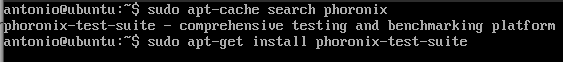
\includegraphics[width=1\textwidth]{imagenes/pho1}
    \caption{Comando para la instalación de Phoronix Suite en Ubuntu.}
    \label{fig1}
  \end{center}
\end{figure}

\begin{figure}[H]
  \begin{center}
    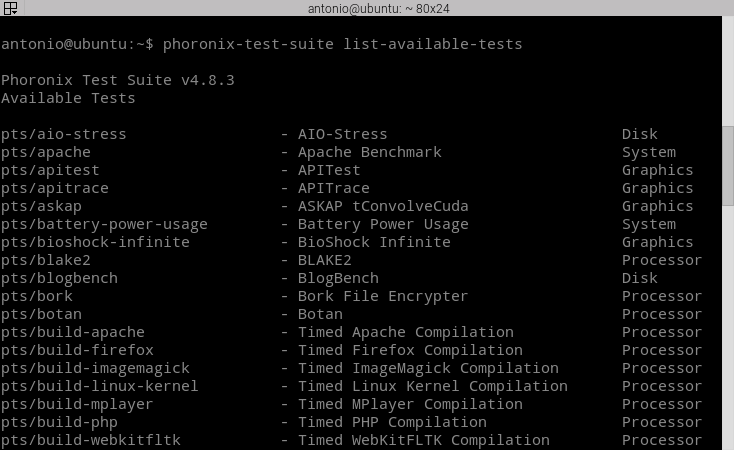
\includegraphics[width=1\textwidth]{imagenes/pho2}
    \caption{Uso del comando \texttt{list-available-tests} para ver los benchmarks disponibles.}
    \label{fig2}
  \end{center}
\end{figure}

\subsection{Cuestión opcional 1}
\textit{Seleccione, instale y ejecute uno, comente los resultados. Atención: no es lo mismo un benchmark que una suite, instale un benchmark.}
\newline

Para esta cuestión he instalado un benchmark llamado pts/n-queen, este benchmark es un programa que usa OpenMP y resuelve el problema de las N-Reinas ( Consiste en colocar un 18 reinas ( en este caso ) en un tablero sin que se amenacen ) en un tablero de tamaño 18 \cite{nr}. La instalación la he realizado como se indica en la \cref{fig13}, los resultados son los mostrados en las \crefrange{fig14}{fig15}.

\begin{figure}[H]
  \begin{center}
    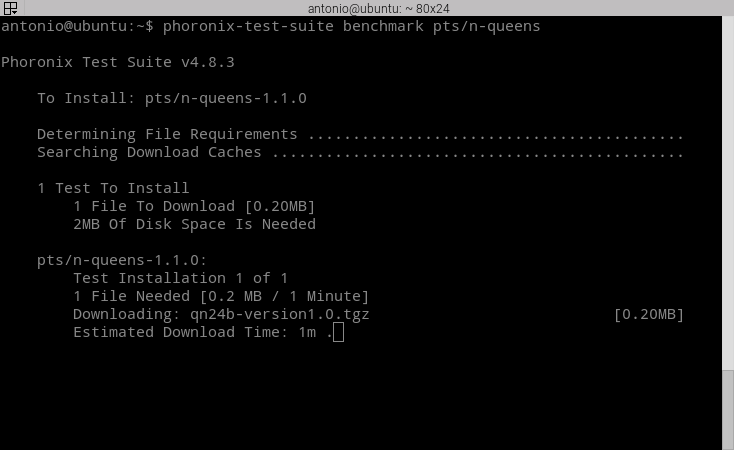
\includegraphics[width=1\textwidth]{imagenes/pho3}
    \caption{Comando para la instalación del benchmark.}
    \label{fig13}
  \end{center}
\end{figure}

\begin{figure}[H]
  \begin{center}
    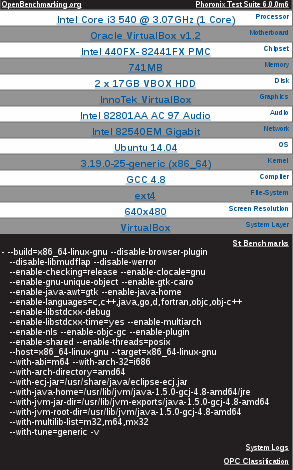
\includegraphics[width=0.4\textwidth]{imagenes/pho4}
    \caption{Información acerca del ordenador usado.}
    \label{fig14}
  \end{center}
\end{figure}

\begin{figure}[H]
  \begin{center}
    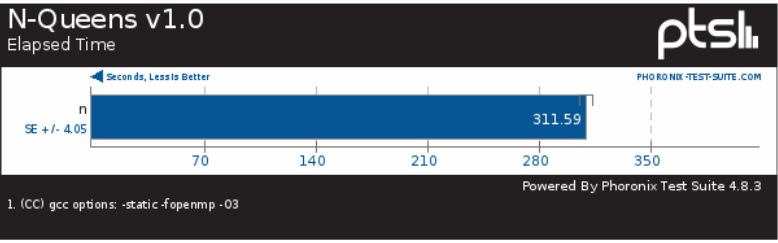
\includegraphics[width=1\textwidth]{imagenes/pho5}
    \caption{Resultado de la ejecución del benchmark, en el resultado se muestra el tiempo medio que se ha invertido en realizar el problema de las N-Reinas.}
    \label{fig15}
  \end{center}
\end{figure}

\section{Benchmarks y tests de estrés para webs}
\subsection{Apache benchmark}

\subsubsection{Cuestión 2}
\textit{De los parámetros que le podemos pasar al comando ¿Qué significa -c 5 ? ¿y -n 100? Monitorice la ejecución de ab contra alguna máquina (cualquiera) ¿cuántos procesos o hebras crea ab en el cliente?}
\newline

El comando \texttt{-c 5} significa que se ejecutaran 5 peticiones concurrentemente y el comando \texttt{-n 100} indica que se van a realizar 100 peticiones al servidor.\cite{ab} En el cliente solo se crea una hebra, como se puede ver con \texttt{top} ( \cref{fig11} ) o mirando en \texttt{/proc/pid\_ab/status} (\cref{fig12}).

\begin{figure}[H]
  \begin{center}
    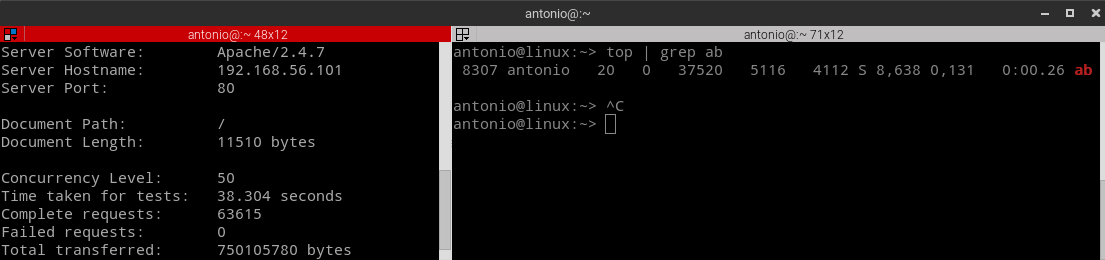
\includegraphics[width=1\textwidth]{imagenes/ab1}
    \caption{Comprobación del número de hebras mediante top.}
    \label{fig11}
  \end{center}
\end{figure}

\begin{figure}[H]
  \begin{center}
    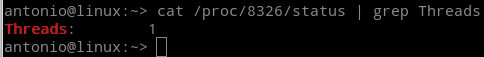
\includegraphics[width=1\textwidth]{imagenes/ab2}
    \caption{Comprobación del número de hebras mediante el archivo /proc/pid\_ab/status.}
    \label{fig12}
  \end{center}
\end{figure}


\subsubsection{Cuestión 3}
\textit{Ejecute ab contra a las tres máquinas virtuales (desde el SO anfitrión a las máquina virtuales de la red local) una a una (arrancadas por separado) y muestre y comente las estadísticas. ¿Cuál es la que proporciona mejores resultados? Fíjese en el número de bytes transferidos, ¿es igual para cada máquina?}
\newline

Para la ejecución del comando \texttt{ab -c 50 -n 100000 ip\_máquina:80/} la que proporciona mejores resultados es la de Windows Server (\cref{fig5})ya que IIS obtiene un rendimiento de 1828,63 peticiones por segundo y tiene un tiempo de respuesta de 0,547 ms, mientras que en Ubuntu ( Apache 2.4.7 ) (\cref{fig3}) se obtiene un rendimiento de 1730,06 peticiones por segundo y un tiempo de respuesta 0,578 ms, en última posición quedaría el servidor con CentOS (Apache 2.2.15 ) (\cref{fig4})  que consigue un rendimiento de 1338,26 peticiones por segundo y un tiempo de respuesta de 0,747 ms.\cite{ab} ( Ver figura \ref{fig6} ). El número de bytes transferido difiere entre las distintas máquinas, esto se debe a que la página solicitada no es igual en todas ellas ( el tamaño se indica en la variable \textbf{Document Length} ), además de que en alguna es posible que los paquetes vayan comprimidos.

\begin{figure}[H]
    \centering
    \begin{subfigure}[b]{0.45\textwidth}
        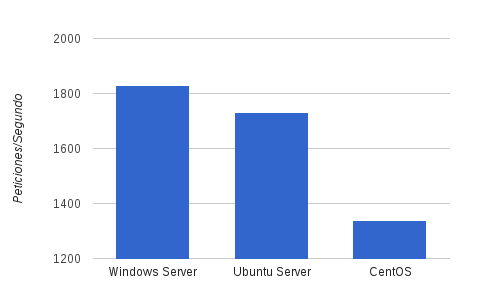
\includegraphics[width=\textwidth]{imagenes/g1}
        \caption{Peticiones por segundo.}
    \end{subfigure}
    \begin{subfigure}[b]{0.45\textwidth}
        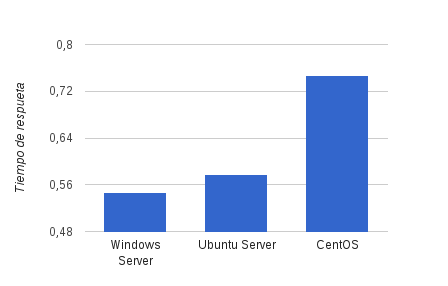
\includegraphics[width=\textwidth]{imagenes/g2}
        \caption{Tiempos de respuesta.}
    \end{subfigure}
    \caption{Comparativa servidores con ab}
    \label{fig6}
\end{figure}

\begin{figure}[H]
  \begin{center}
    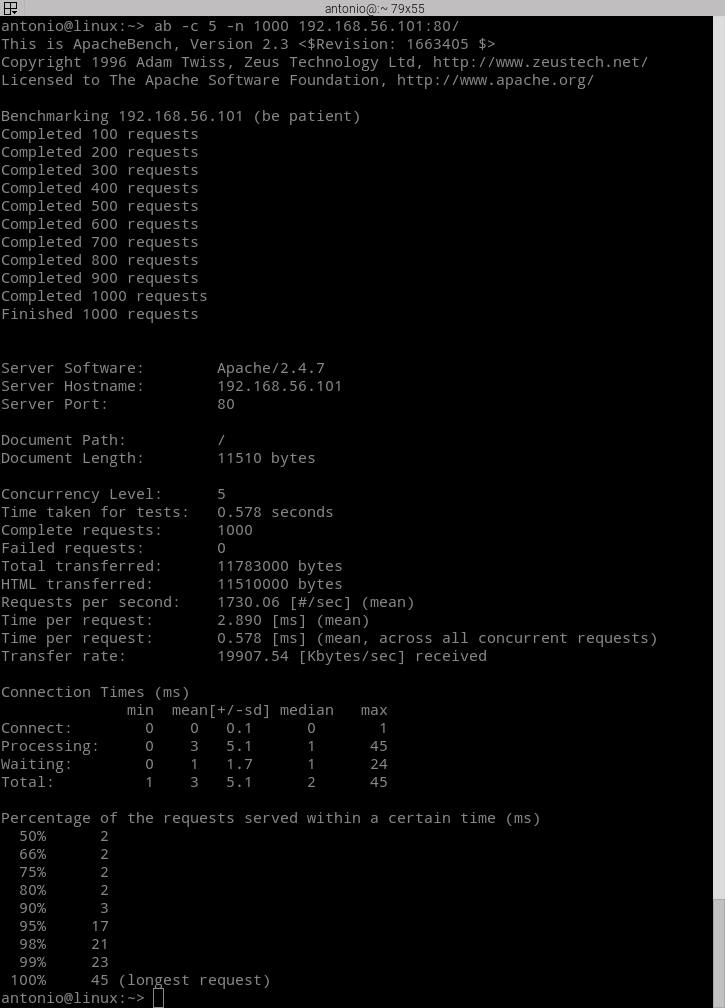
\includegraphics[width=1\textwidth]{imagenes/abub}
    \caption{Resultado de la ejecución de ab contra la maquina virtual de Ubuntu Server.}
    \label{fig3}
  \end{center}
\end{figure}
\begin{figure}[H]
  \begin{center}
    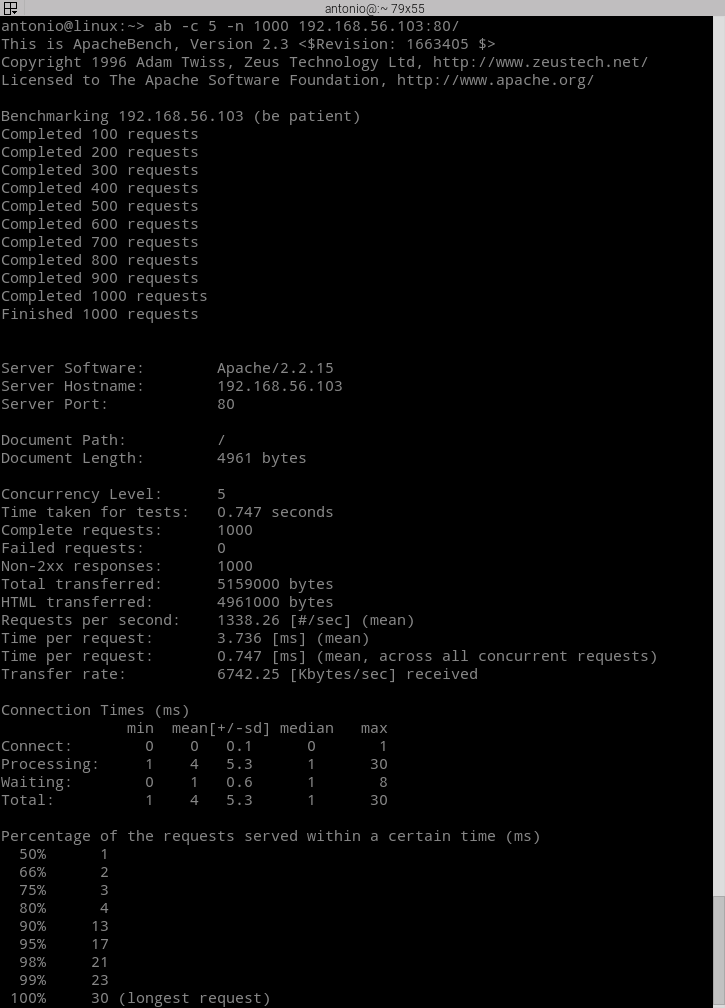
\includegraphics[width=1\textwidth]{imagenes/abce}
    \caption{Resultado de la ejecución de ab contra la maquina virtual de CentOS.}
    \label{fig4}
  \end{center}
\end{figure}
\begin{figure}[H]
  \begin{center}
    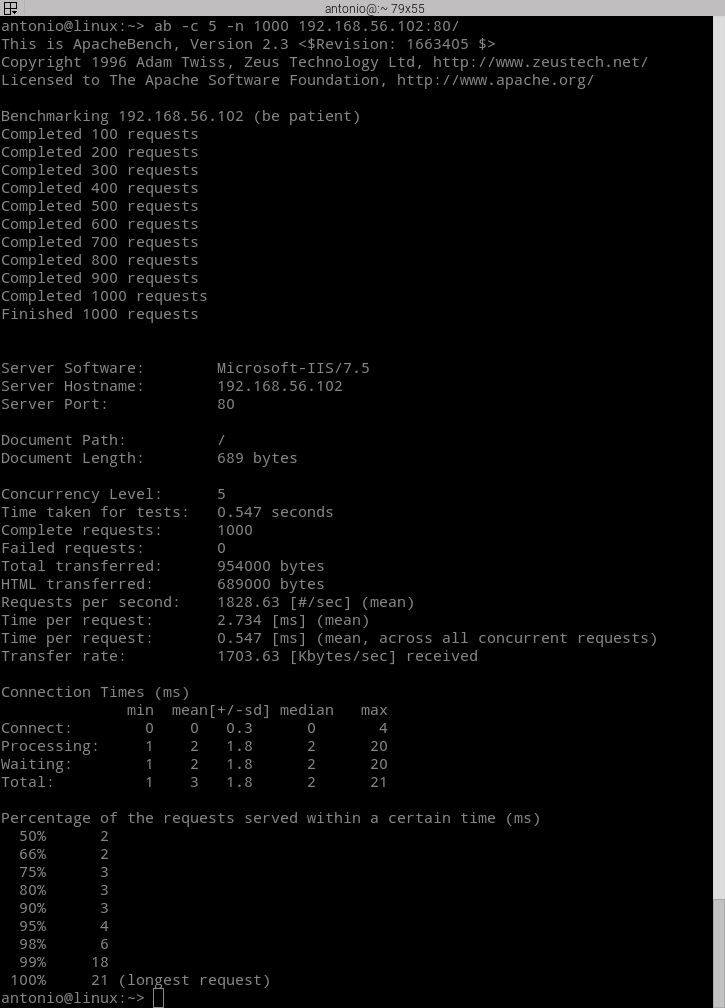
\includegraphics[width=1\textwidth]{imagenes/abwin}
    \caption{Resultado de la ejecución de ab contra la maquina virtual de Windows Server.}
    \label{fig5}
  \end{center}
\end{figure}


\subsection{Jmeter}

\subsubsection{Cuestión 4}
\textit{Instale y siga el tutorial en \url{http://jmeter.apache.org/usermanual/build-web-test-plan.html} realizando capturas de pantalla y comentándolas. En vez de usar la web de jmeter, haga el experimento usando alguna de sus máquinas virtuales (Puede hacer una página sencilla, usar las páginas de phpmyadmin, instalar un CMS, etc.).}
\newline

Para realizar esta cuestión, en primer lugar, debemos conseguir JMeter, esto se puede hacer de dos formas, descargando el programa de \cite{jm} o mediante la orden \texttt{sudo apt-get install jmeter} en Ubuntu. Si optamos por el primer método deberemos extraer el archivo descargado y dentro, en la carpeta /bin, ejecutar \texttt{./jmeter.sh}. Una vez que tenemos JMeter funcionando podemos proceder a seguir el tutorial disponible en la web de JMeter \cite{tut}, en mi caso voy a realizar peticiones a phpMyAdmin. El proceso de configuración se puede ver en las \crefrange{fig7}{fig10}.

\begin{figure}[H]
  \begin{center}
    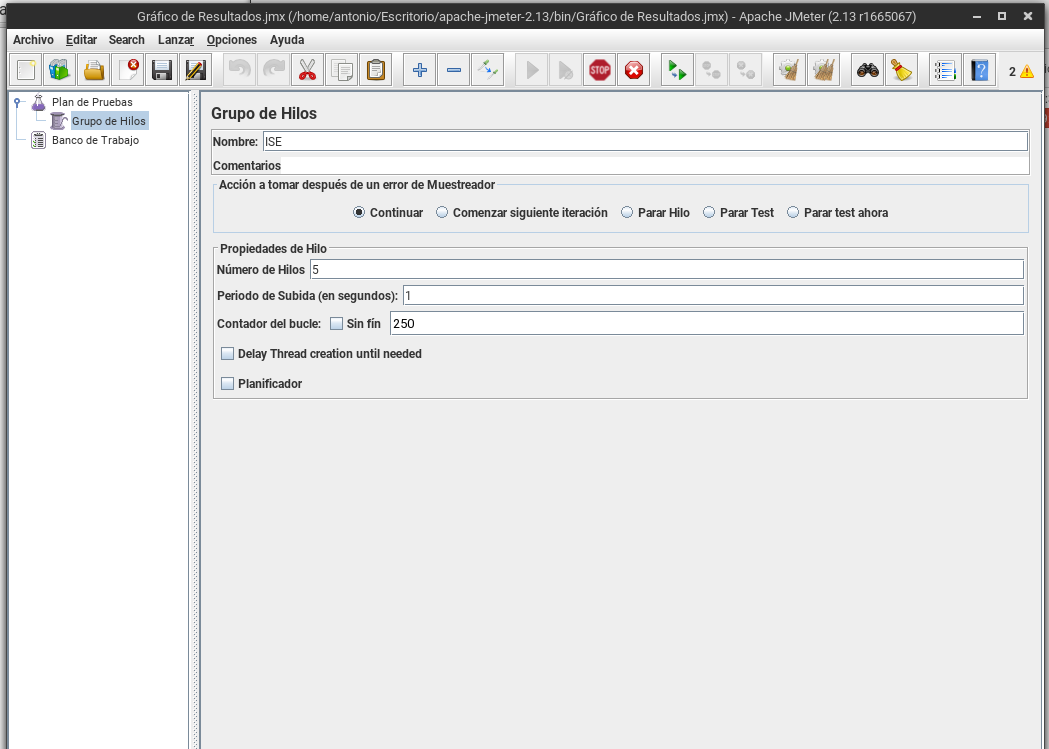
\includegraphics[width=0.7\textwidth]{imagenes/jm1}
    \caption{Añadimos un grupo de threads ( Thread Group o Grupo de Hilos ) que simularan los usuarios, en esta caso se configuran 5 usuarios y se repetirá el 250 veces.}
    \label{fig7}
  \end{center}
\end{figure}

\begin{figure}[H]
  \begin{center}
    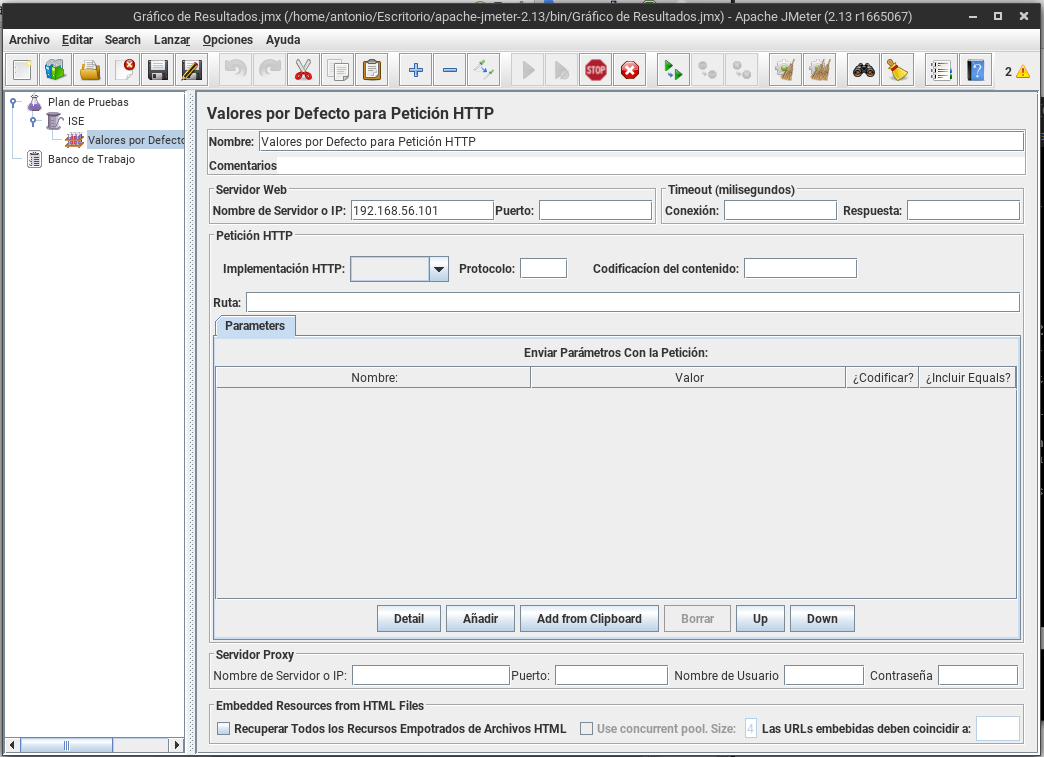
\includegraphics[width=0.7\textwidth]{imagenes/jm2}
    \caption{Añadimos los valores por defecto para las peticiones HTTP, en este caso de indica la IP de mi servidor.}
    \label{fig8}
  \end{center}
\end{figure}

\begin{figure}[H]
  \begin{center}
    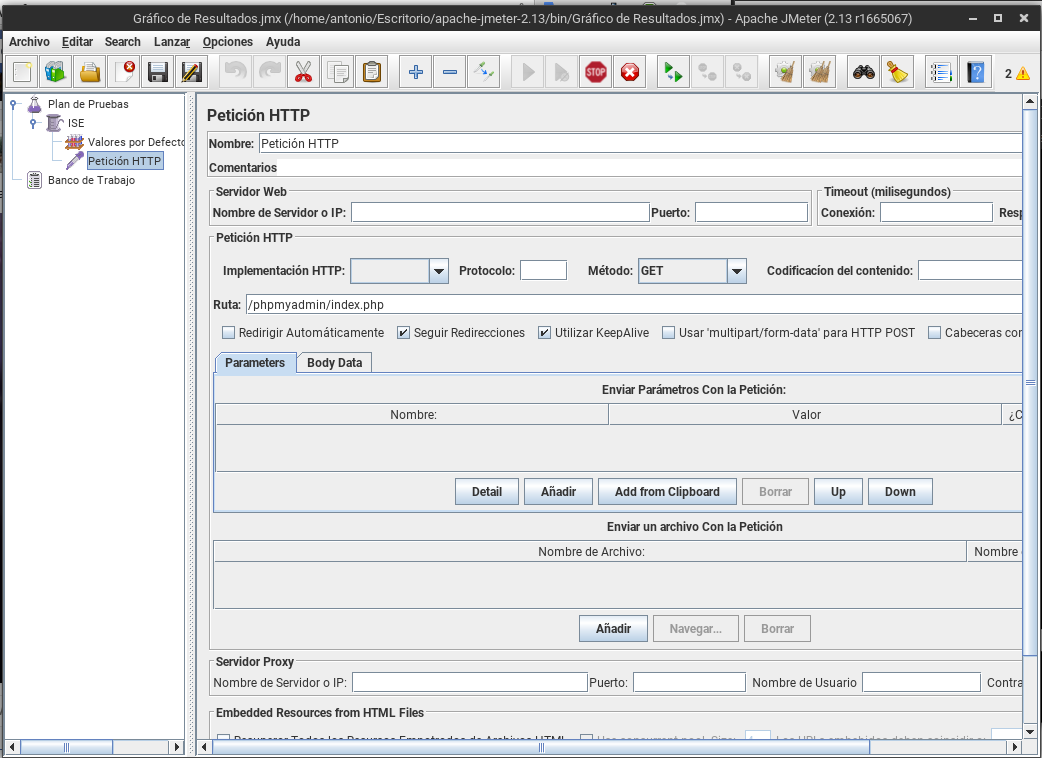
\includegraphics[width=0.7\textwidth]{imagenes/jm3}
    \caption{Se añade la petición HTTP que se va a realizar, en este caso un petición a la pagina de login de phpMyAdmin.}
    \label{fig9}
  \end{center}
\end{figure}

\begin{figure}[H]
  \begin{center}
    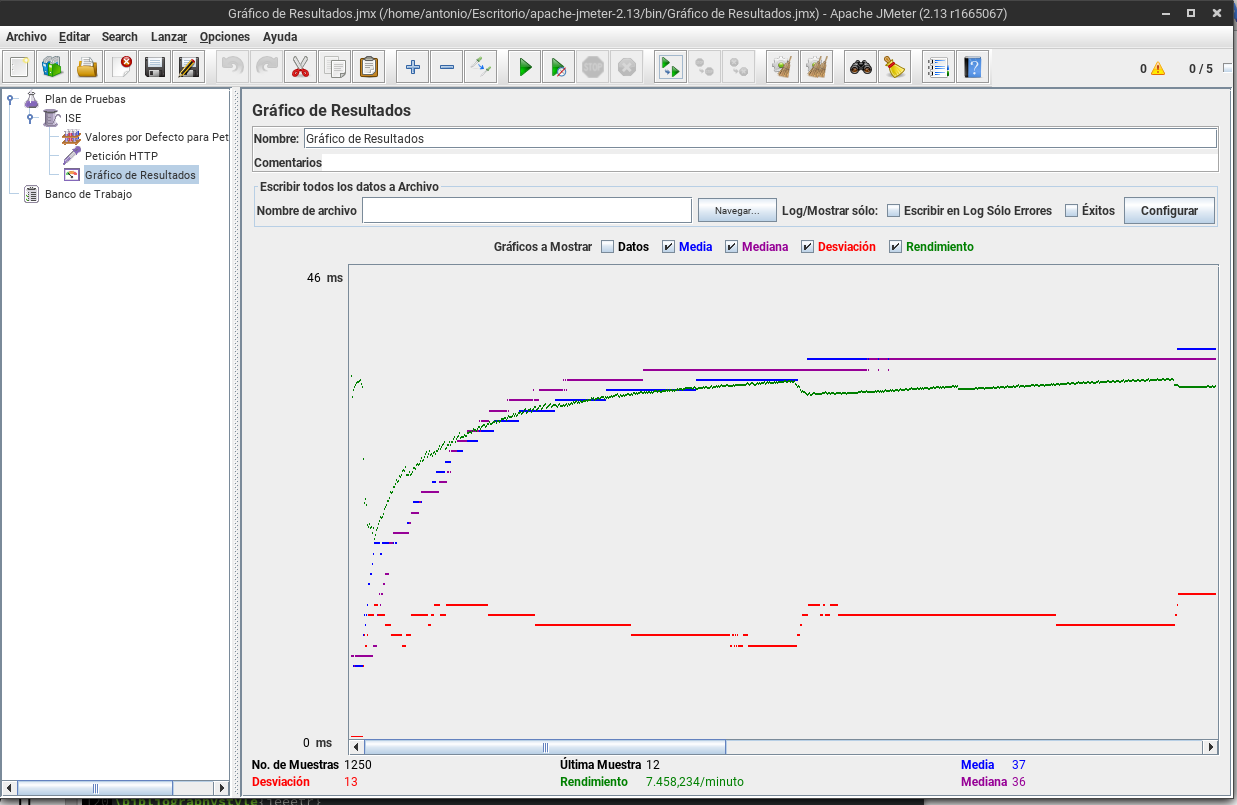
\includegraphics[width=0.7\textwidth]{imagenes/jm4}
    \caption{Añadimos un gráfico de resultados para poder ver el resultado de la ejecución del test. En este caso se puede ver que al principio el rendimiento del servidor va subiendo y luego se estabiliza.}
    \label{fig10}
  \end{center}
\end{figure}



\section{Benchmarks para Windows}
\subsection{AIDA64 (Antiguo Everest)}

\subsubsection{Cuestión opcional 4}
\textit{Seleccione un benchmark entre SisoftSandra y Aida.
Ejecútelo y muestre capturas de pantalla comentando los resultados.}
\newline

En primer lugar he instalado SisoftSandra y Aida, ambas instalaciones han sido bastante simples. Luego he ejecutado un benchmark llamado CPU PhotoWorxx que realiza operaciones comunes de manipulación de imágenes sobre un imagen muy grande \cite{aida} ( \cref{aida} ) en el se muestra información acerca del ordenador y cuantos  megapixeles se han procesado por segundo. Por otro lado he ejecutado un benchmark de aritmética del procesador en SisoftSandra, este benchmark muestra una enorme cantidad de información ( \cref{sandra} )  entre la que se incluye la información de rendimiento, rendimiento frente a energía y rendimiento frente a velocidad.

\begin{figure}[H]
  \begin{center}
    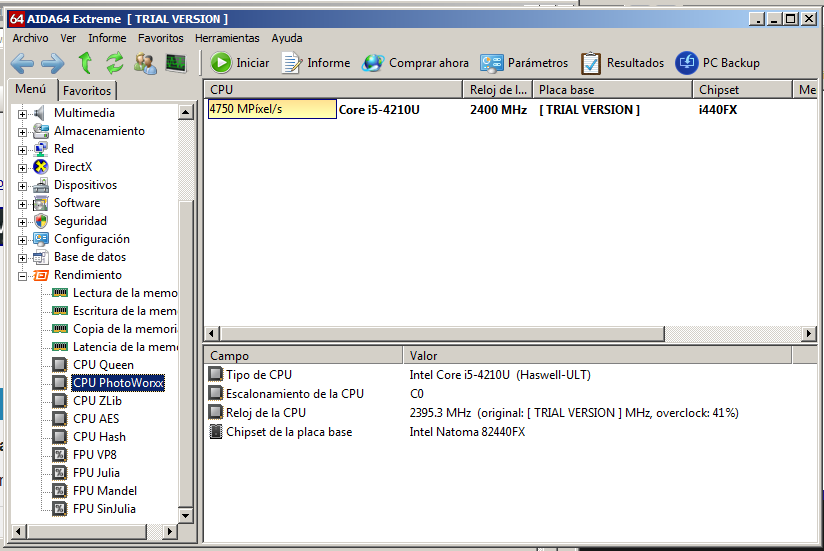
\includegraphics[width=0.7\textwidth]{imagenes/aida}
    \caption{Ejecucion del benchamark CPU PhotoWorxx en Aida.}
    \label{aida}
  \end{center}
\end{figure}

\begin{figure}[H]
  \begin{center}
    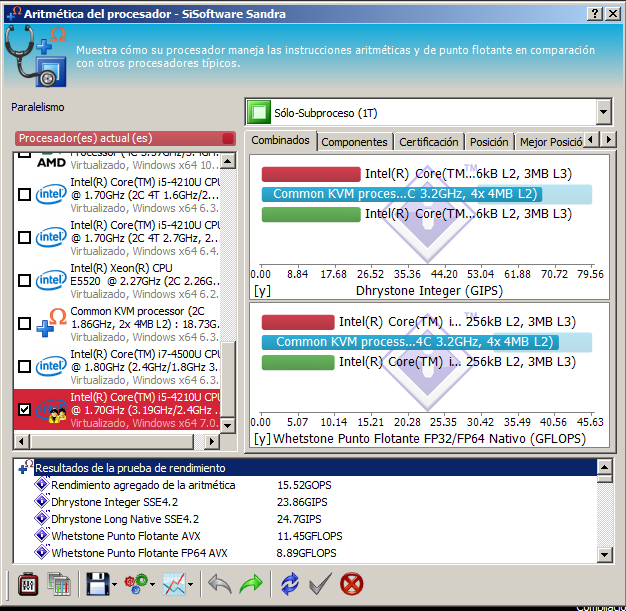
\includegraphics[width=0.7\textwidth]{imagenes/sandra}
    \caption{Ejecución del benchmark de aritmética de Sandra.}
    \label{sandra}
  \end{center}
\end{figure}

\section{Más benchmarks}
\subsection{Cuestión 5}
\textit{Cuestión 5: Programe un benchmark usando el lenguaje que desee. El benchmark debe incluir:
\begin{enumerate}
  \item Objetivo del benchmark
  \item Métricas (unidades, variables, puntuaciones, etc.)
  \item Instrucciones para su uso
  \item Ejemplo de uso analizando los resultados
\end{enumerate}}

\begin{enumerate}
  \item El objetivo del benchmark realizado es obtener unos tiempos para poder comparar distintas CPU sin que se tenga que hacer uso de RAM y disco duro, para que esos componentes no afecten al resultado del rendimiento de la CPU, el benchmark, consiste en el cálculo de PI haciendo uso de la integral: $$ \pi = \int_{0}^{1} \frac{4}{1+x^{2}} $$ Esta cálculo se lleva a cabo de forma secuencial y de forma paralela. He elegido este cálculo porque es apto para ser paralelizado y además no se necesita guardar muchos datos, por lo que el uso de memoria RAM será mínimo.
  
  \item La ejecución del benchmark devuelve dos aproximaciones de $\pi$ , que no tienen interés a la hora de comparar las CPU y además devuelve \textbf{dos tiempos}, uno de la \textbf{ejecución secuencial} y otro de la \textbf{ejecución en paralelo}. El tiempo de la ejecución secuencial, nos indica el tiempo que ha tardado la realización del cálculo haciendo uso de una sola hebra, por lo tanto nos permite comparar que CPU es más rápida para la ejecución de aplicaciones secuenciales, el otro tiempo mostrado, es el requerido para hacer el cálculo en paralelo haciendo uso de todas las hebras del procesador, lo que nos permite comparar que CPU tiene un mayor rendimiento total y para aplicaciones paralelas.
  
  \item Para usar este benchmark en primer lugar hay que compilarlo mediante la orden \texttt{``g++ -fopenmp benchmark.cpp -o benchmark''}, tras la compilación se puede ejecutar mediante \texttt{``./benchmark''}. Una vez que lo ejecutamos nos pide el número de iteraciones que se van a llevar a cabo para el cálculo de $\pi$ , y luego se pregunta por el número de veces que se va a realizar el cálculo, cuanto mayor sea este número, el valor del tiempo se ajustará mejor a la realidad ya que se realizará la media de los tiempos tomados en más ocasiones.
  
  \item Para mostrar el uso del benchmark he realizado las ejecuciones mostradas en la \cref{fig16} y en la \cref{fig17}. Tras mirar los tiempos del benchmark podemos ver que la CPU \texttt{ Pentium Dual-Core E5400} ( \cref{fig16} ) obtiene un mejor tiempo para el uso de una sola hebra (algo que cabía esperar dado que su frecuencia de reloj es muy superior a la de la otra CPU) por lo que podríamos decir que la CPU\texttt{ Pentium Dual-Core}, es mejor que la otra CPU para la ejecución de una aplicación que solo use una hebra. En cambio el tiempo obtenido por la CPU \texttt{Intel Core i5 4210U}( \cref{fig17} ) para la ejecución paralela es mejor que el de la CPU\texttt{ Pentium Dual-Core}, probablemente porque la CPU \texttt{Intel Core i5} tiene cuatro hebras y la otra solo tiene dos, por lo cual podemos concluir que la CPU \texttt{Pentium Dual-Core E5400} es mejor para al ejecución de una aplicación que requiera de una sola hebra, mientras que la CPU \texttt{Intel Core i5 4210U} es mejor en caso de que la aplicación use múltiples hebras.
\end{enumerate}

\begin{figure}[H]
  \begin{center}
    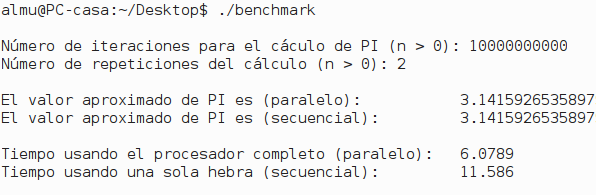
\includegraphics[width=1\textwidth]{imagenes/bench1}
    \caption{Ejecución del benchmark en un ordenador con una CPU Intel\textregistered\ Pentium\textregistered\ Dual-Core E5400 a 2,7GHz.}
    \label{fig16}
  \end{center}
\end{figure}

\begin{figure}[H]
  \begin{center}
    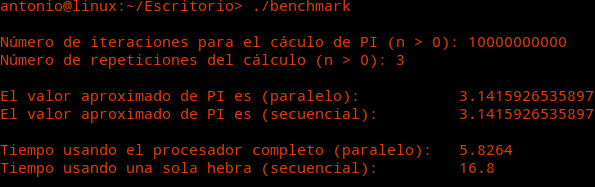
\includegraphics[width=1\textwidth]{imagenes/bench2}
    \caption{Ejecución del benchmark en un ordenador con una CPU Intel\textregistered\ Core\texttrademark\ i5 4210U CPU a 1.70GHz.}
    \label{fig17}
  \end{center}
\end{figure}
%*************************************************************
\newpage
\bibliographystyle{ieeetr}
\bibliography{citas}

\end{document}
